\documentclass[12pt,letterpaper]{report}

% PAQUETES UTILIZADOS
\usepackage[spanish]{babel}
\usepackage{cite}
\usepackage[utf8]{inputenc}
\usepackage{graphicx}
\usepackage{mathrsfs}
\usepackage{enumitem}
\usepackage{float}
\usepackage{researchdiary_png}
\usepackage{subfig}
\newcommand{\workingDate}{\textsc{ }}
\newcommand{\userName}{ }
\newcommand{\institution}{ }



%////////////// Inicio del documento //////////////

\begin{document}

\begin{titlepage}
\centering
%////////////// PORTADA //////////////
\begin{center}

\includegraphics[scale=0.5]{uaem_logo.png}
\end{center}
\vspace{0.5cm}
{\bfseries\normalsize UNIVERSIDAD AUTÓNOMA DEL ESTADO DE MORELOS\newline
INSTITUTO DE INVESTIGACIÓN EN CIENCIAS BÁSICAS Y APLICADAS\newline 	
CENTRO DE INVESTIGACIÓN EN CIENCIAS
 \par}
\vspace{1.5cm}
{\scshape\Huge\bfseries MS-2k1 \par}
\vspace{1.5cm}
{\bfseries\scshape\Large REPORTE \par}
\vspace{0.3cm}
{\Large{INTRODUCCIÓN A LA PROGRAMACIÓN DE VIDEOJUEGOS EN C++ Y PYTHON}}\\
\vspace{0.3cm}
\vspace{1.5cm}
{\Large PRESENTA \\}
\vspace{0.3cm}
{\bfseries\scshape\Large\textit{ANDRÉS REYES - FRANCISCO AQUINO - EDUARDO NUÑEZ}\par}
\vspace{1cm}
\Large PROFESOR: \\
\vspace{0.2cm}
\itshape\Large\bfseries Mtro. Yainier Labrada Nueva \par

\end{titlepage}

%////////////// TABLA DE CONTENIDOS //////////////
\tableofcontents
%====================================================================================
%
%
% CAPITULO 1: INTRODUCCION
%
%
%
\chapter{Introducción} %Capitulos

En los últimos años, la industria de los videojuegos se ha visto envuelta en una revolución tecnológica abismal, el poder de computo y las ascendentes tecnologías en el área de la comunicación digital, han abierto puertas inmensas para todas las ramas de tecnología en el mundo, entre ellas, el desarrollo de videojuegos.

Los videojuegos recrean entornos y situaciones virtuales en los que la persona puede controlar a uno o mas personajes de este entorno. 

Este proyecto tiene el enfoque de poder aprender y analizar la programación de videojuegos, que emplea muchos paradigmas de la programación como la programación orientada a objetos, a eventos, procesos, y muchos conceptos más. \cite{Inventa}

\section{Videojuegos}

Los videojuegos, como concepto, se componen por distintas partes, una de ellas es el controlador, que es un dispositivo de entrada que varía dependiendo de la plataforma. Por ejemplo, un controlador podría consistir únicamente de un botón y una palanca, mientras que otros podrían tener más de una docena de botones y una o más palancas.


%====================================================================================
%
%
% CAPITULO 1: INTRODUCCION Y OBJETIVOS
%
%
%

\chapter{Objetivos}
\textit{Veni vidi vici.}

\section{Objetivos específicos}

Esta sección esta enfocada a las distintas metas que se propusieron alcanzar como base para la realización de este proyecto. Las siguientes son:

\begin{itemize}

\item Adquirir las bases y el conocimiento para poder desarrollar un videojuego desde cero.

\item Comprender como se emplea la programación y la lógica en algo tan complejo como lo es un videojuego.

\item Entender la modelación y aplicación de la programación orientada a objetos en un sistema en tiempo real, con eventos y objetos en constante cambio, dentro de un entorno simulado.

\end{itemize}


\section{Objetivos generales}

Los objetivos enlistados aquí, son metas que sobre la marcha, se vislumbraban completables a lo largo del desarollo del videojuego. Algunas de ellas son:

\begin{itemize}

\item Aprender y reforzar un lenguaje de programación de alta popularidad como lo es Python\cite{Python}.

\item Aplicar y desarrollar conceptos adquiridos en la formación académica en un proyecto real e integral.

\item Desarrollar y pulir las distintas habilidades de programación que se han adquirido a lo largo de la formación académica.


\end{itemize}


%====================================================================================
%
%
%
% CAPITULO 2: MARCO TEORICO
%
%
%



\chapter{Marco teórico}

El marco teórico que presentamos aquí basado en una exhaustiva investigación para poder corroborar cuales eran los mejores métodos para implementar el proyecto.

\section{Anaconda\cite{Anaconda}} 

Anaconda es una distribución libre y abierta de los lenguajes Python y R. Utilizamos anaconda por su flexibilidad y por su completud en cuanto a entornos concierne, el ecosistema de Python permite hacer instalación de paquetes de una forma  muy sencilla y rápida. 

Dentro de Anaconda utilizamos JupyterLab, que es una herramienta que nos permite visualizar y editar el código por celdas, manteniendo un mejor control de los errores.



\section{Python\cite{Python}} 

Python es un lenguaje de programación de alto nivel, muy sencillo de aprender a utilizar, y además es multiparadigma, por lo que Python se presta para realizar cualquier tipo de tarea, como es el caso: un videojuego.

Es un lenguaje de programación versátil, utilizado en muchas áreas, como lo son la estadística, la comunicación y la ciencia de datos. 

Algunas de sus ventajas son:

\begin{itemize}

\item Es simple y rapido: puedes hacer mucho con pocas lineas de código.

\item Flexible: No necesariamente vas a tener que preocuparte por detalles de tipificación y declaraciones.

\item Multiplataforma: Se puede ejecutar en cualquier sistema operativo y cuenta con librerías especificas para cada uno de estos.

\item Open Source: Su comunidad se encarga de mantener al lenguaje y crear todos sus recursos de forma gratuita.


\end{itemize}



\section{Pygame\cite{Pygame}} 

Pygame es un conjunto de módulos del lenguaje Python que permiten y facilitan la creación de videojuegos en dos dimensiones de una manera sencilla, gracias al manejo de sprites.

Este conjunto de modulos, permite una flexibilidad y manejo en la manipulación de sprites.

\subsection{Sprites}


Los sprites sirven para la optimización del uso de imágenes empleadas en CSS. Mediante la construcción de una cuadricula de imagenes ordenadas y el uso de estilos, se pueden ubicar todas las imagenes mostrando solo una porción de la imagen. Esto optimiza tiempos de descarga de una página como rendimiento de las mismas.
\\ \\ \\
\begin{figure}[h]
\begin{center}

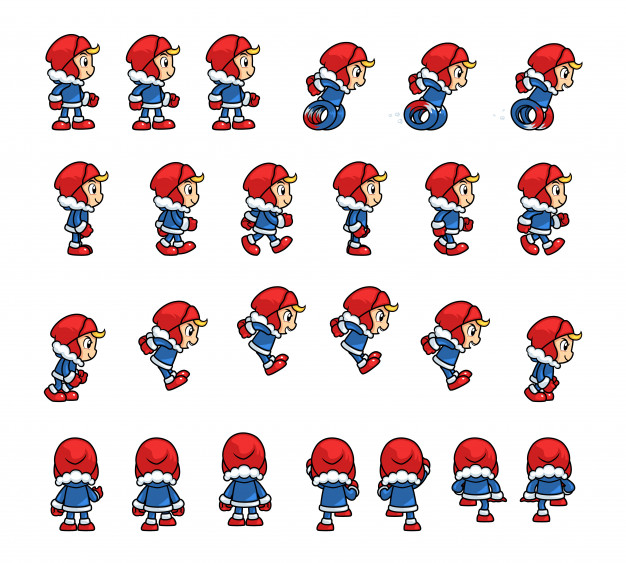
\includegraphics[scale=0.5]{../../SecondGame/esquimal.jpg} 
\caption{Ejemplo de sprites}
\end{center}
\end{figure}


\chapter{Composición y desarrollo}
\textit{Augere.}

\section{Nociones básicas del juego desarrollado}

El presente proyecto es un videojuego desarrollado en el lenguaje de programación Python, haciendo uso de los módulos de Pygame; el cual esta diseñado para dos jugadores simultáneos los cuales controlan dos naves espaciales en un enfrentamiento y gana aquel jugador que terminé primero con las vidas del oponente.

\section{Partes integrales del juego}
El videojuego se compone de tres partes principales, las cuales son:

\subsection{Pantalla}
La pantalla principal del juego es un fondo estático de dimensiones 900x500 pixeles, sobre el cual se dibujan los demás componentes del juego. Como imagen de fondo se uso una foto del Centro de Investigación en Ciencias convertida a negativo, como se muestra a continuación:
\begin{center}
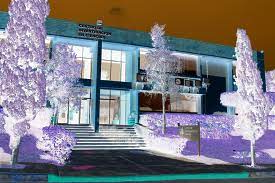
\includegraphics[scale=0.5]{negative_cinc.png} 
\end{center} 
Dicha imagen se divide a la mitad con el próposito de asignar a cada jugador ese espacio que actua como su aréa de juego desde el cual ninguno de los dos se puede mover afuera de la misma.\newline
En las esquinas superiores se dibujan a manera de texto las vidas restantes de cada jugador, las cuales se decrementan si un jugador ha sido impactado por una bala del oponente. 
\begin{center}
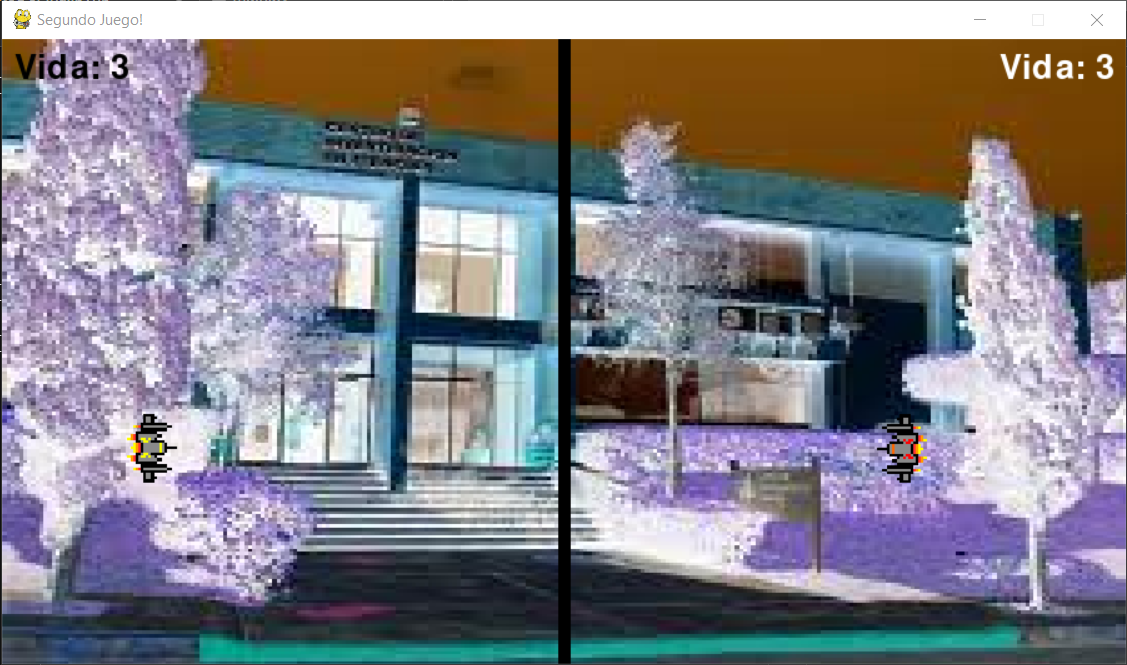
\includegraphics[scale=0.75]{execute_order_66.png} 
\end{center}




\subsection{Naves}
Las naves están compuestas de imágenes tipo PNG de 100x300 pixeles. En ambas naves predomina el color gris con contorno negro, tienen también colores rojos, naranjas y amarillos para simular fuego saliendo de los motores. 

Una de ellas tiene señas de color rojo mientras que la otra las tiene de color amarillo, como se muestra en la siguiente imagen:
\begin{center}
\begin{figure}[h]
 \centering
  \subfloat[Jugador 1]{
   \label{f:jugador1}
	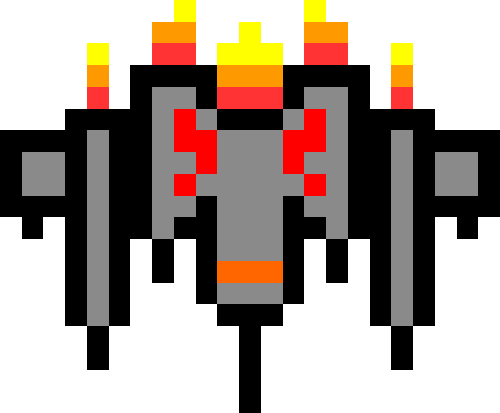
\includegraphics[scale=0.3]{spaceship_red.png}}
  	\subfloat[Jugador 2]{
   	\label{f:jugador 2}
	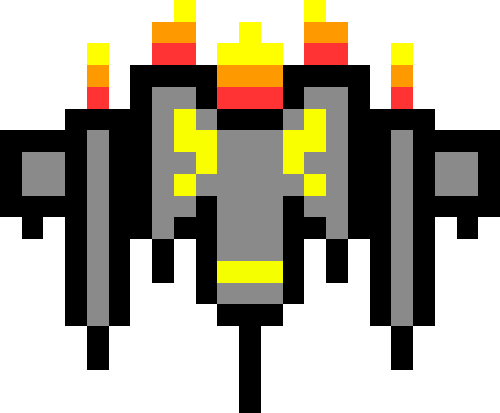
\includegraphics[scale=0.3]{spaceship_yellow.png} }
 \caption{Naves}
 \label{f:naves}
\end{figure}
\end{center}

\chapter{Conclusiones}
\textit{In termino.} \\ \\ \\ 
Al finalizar este proyecto pudimos lograr comprender de una mejor manera todo el trabajo que conlleva crear un videojuego, así como la lógica detrás de la escritura del código y la manera en la que se debe de observar un juego desde la prespectiva de un desarrollador, es decir, ver el programa tomando en cuenta el paradigma de programación orientada a objetos. \newline\newline
Pudimos obervar cómo se van actualizando y modificando los elementos del programa con cada ciclo temporal que pasaba. \newline \newline
También logramos reforzar nuestros conocimientos sobre la programación en Python. Este lenguaje de programación nos ayudó mucho a la realización del programa dada la facilidad que tiene de utilizarse para el paradigma de programación orientada a objetos. Además de ser un lenguaje de programación muy utilizado actualmente, esto significa que al poner en práctica nuestra escritura de código en este lenguaje nos prepara un poco más para nuestro futuro como programadores. \newline\newline
Nos dimos cuenta de que los conocimientos previamente adquiridos a lo largo de nuestra carrera se conjuntaron para ayudarnos a entender y así realizar el proyecto con mucha más facilidad.

\begin{thebibliography}{0}

  \bibitem{Inventa} Sweigart, A. (2015). Inventa tus Propios Juegos de computadora con Python. Libro Version ES. 0.1.
    
  \bibitem{Anaconda} https://www.anaconda.com/
  
  \bibitem{Python} https://www.python.org/
  
  \bibitem{Pygame} https://www.pygame.org/docs/  
  
  
\end{thebibliography}

\end{document}